\section{Introduction}
Due to the emergence of large language models (LLMs), the `pre-train, prompt, and predict' paradigm has revolutionized natural language processing (NLP) in real-world applications, such as open-domain question answering, fact-checking, and arithmetic reasoning~\cite{chen2017reading, thorne2018fever, asai2019learning, karpukhin2020dense, aly2021feverous, qin2023chatgpt, zou-caragea-2023-jointmatch, liu2023tackling}. However, no significant efforts have investigated this framework in the scenario of multi-documental question answering (MD-QA), which enjoys practical usage in academic research, customer support, and financial/legal inquiries that require deriving insightful analysis from multiple documents~\cite{tessuto2011legal, bolino2016impression}.

\begin{figure}[t!]
    \centering
    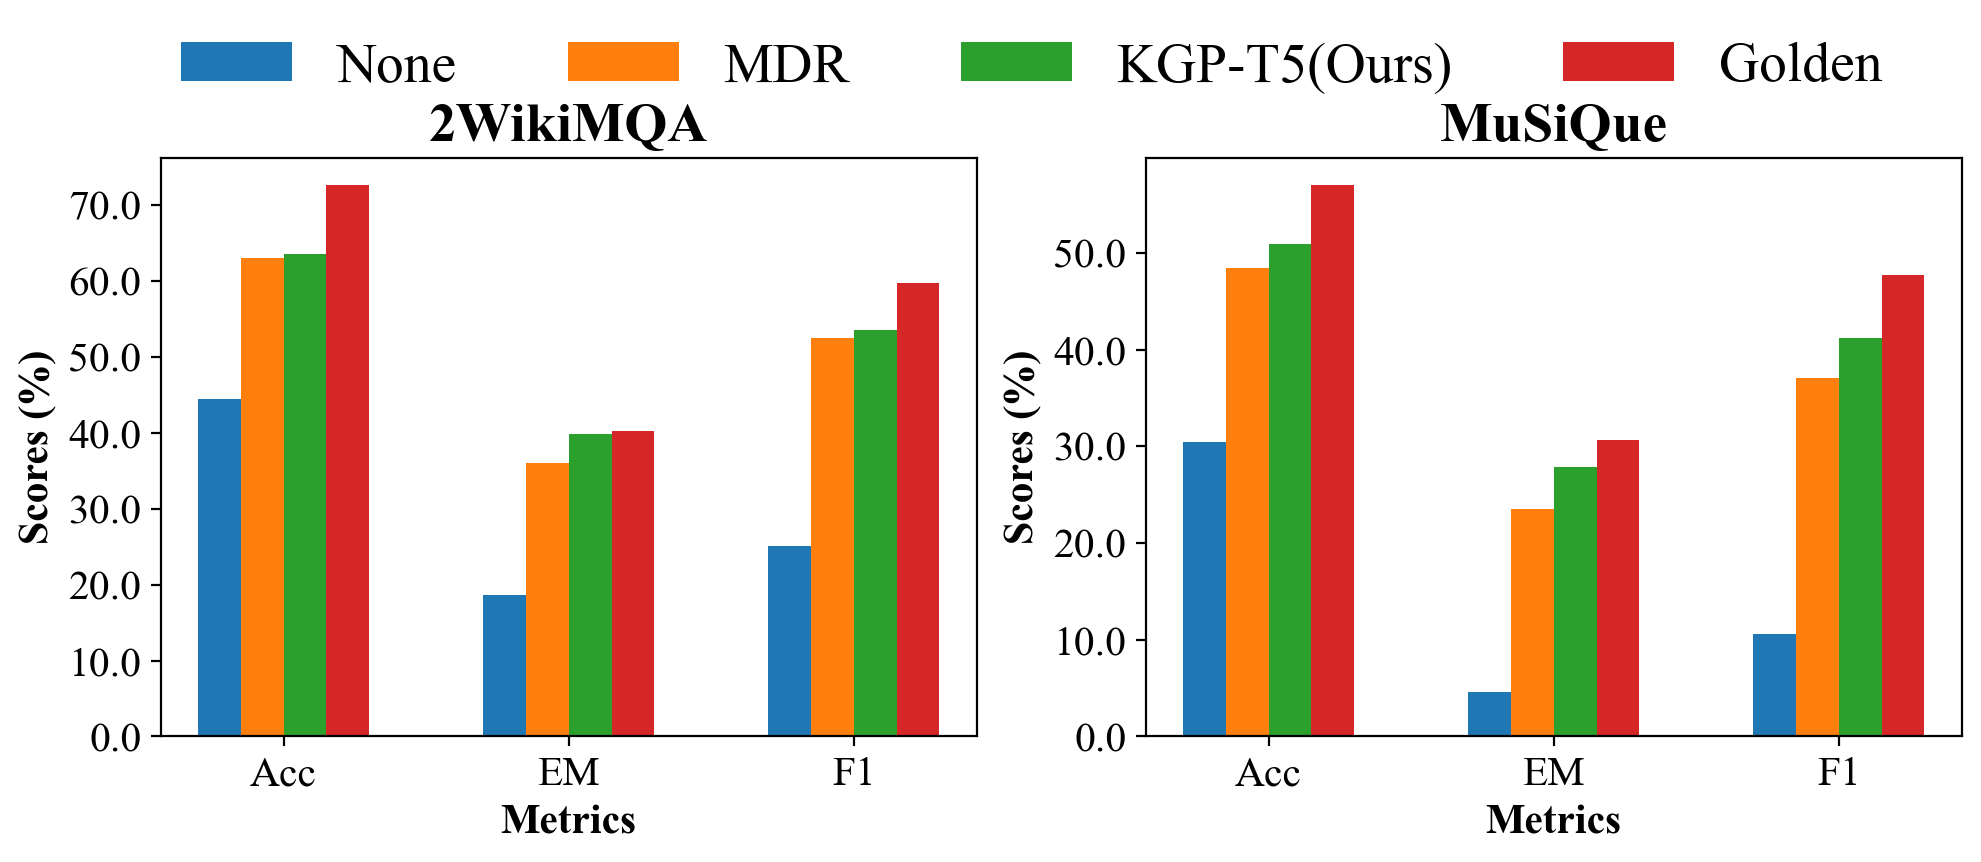
\includegraphics[width=0.5\textwidth]{Figure/motivation_perform.png}
    \caption{MD-QA performance when prompting ChatGPT with the context retrieved using different strategies.}
    \label{fig-motivate_perform}
    \vspace{-3ex}
\end{figure}

\begin{figure*}[t!]
    \centering
    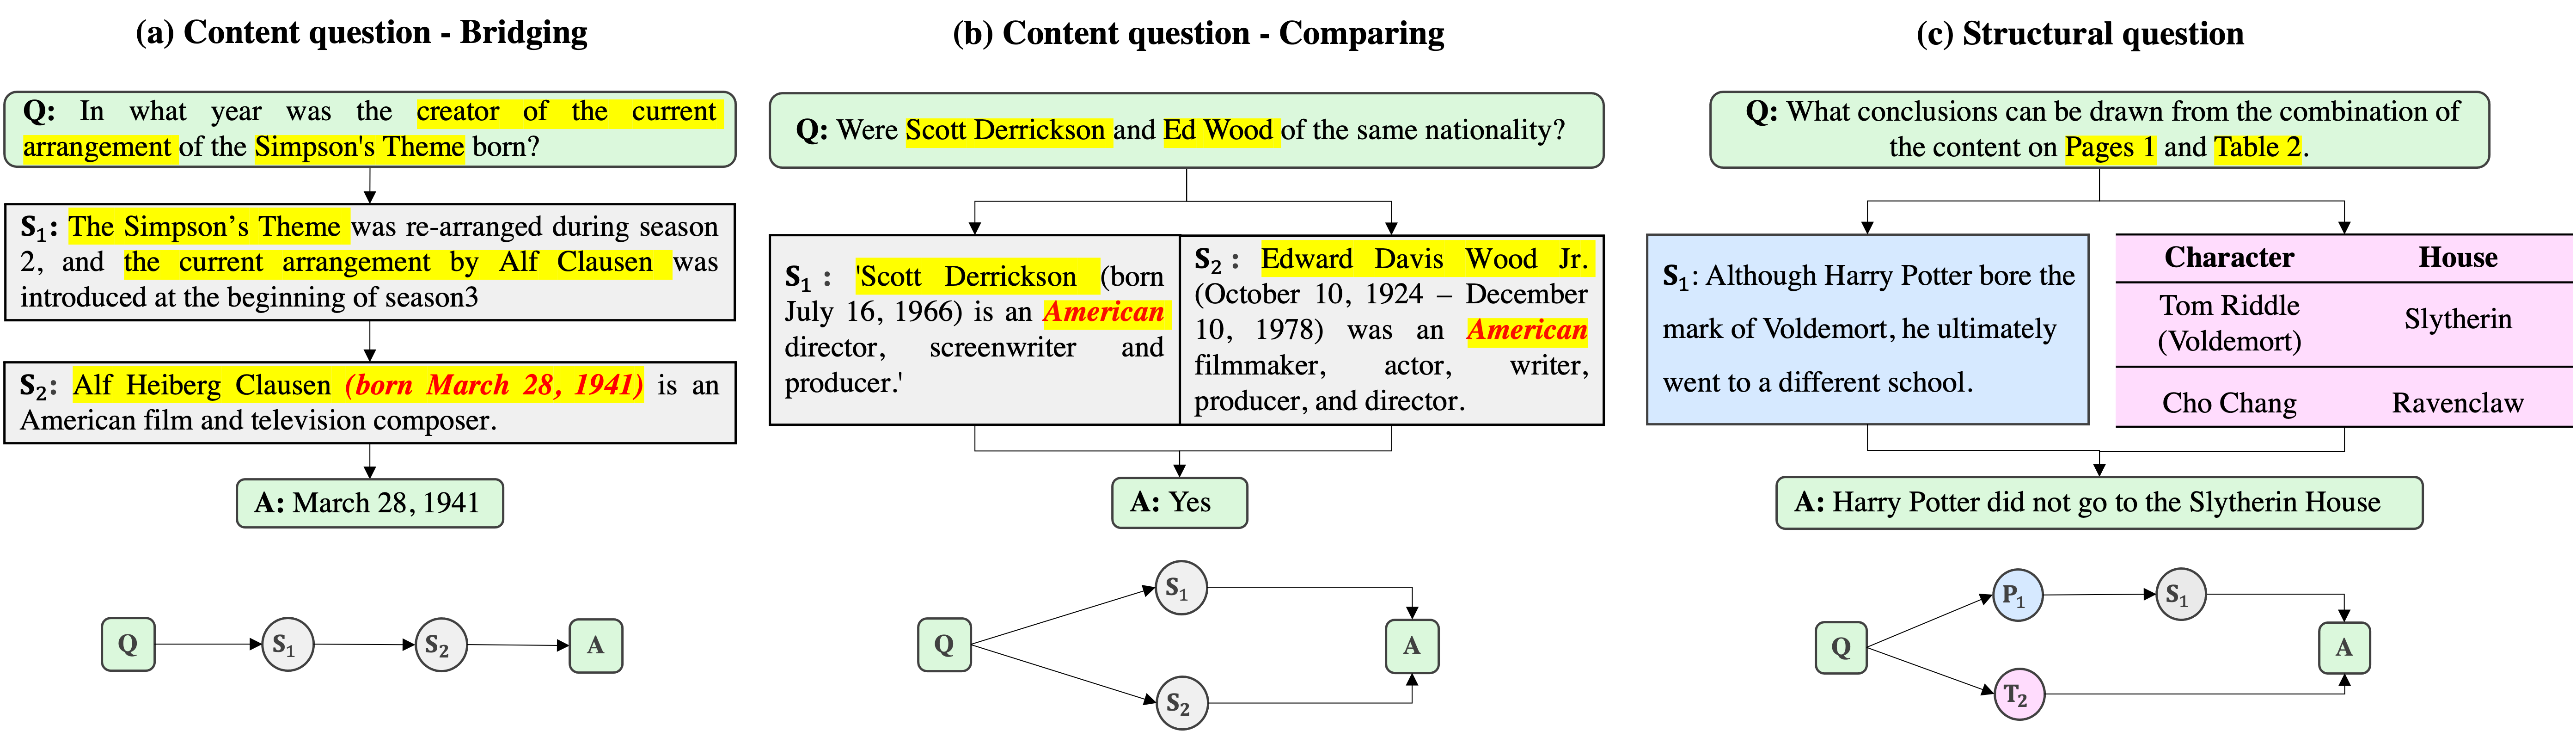
\includegraphics[width=1\textwidth]{Figure/motivation.png}
    \caption{Three popular questions that require reasoning and retrieving over passages/pages/tables from multiple documents. \textbf{(a) Bridging questions} rely on sequential reasoning while \textbf{(b) Comparing questions} rely on parallel reasoning over different passages. \textbf{(c) Structural questions} rely on fetching contents in the corresponding document structures.}
    \label{fig-question}
    \vspace{-2ex}
\end{figure*}

To investigate the capability of LLMs for MD-QA, we randomly sample multi-document questions from the development set of 2WikiMQA~\cite{ho2020constructing} and MuSiQue~\cite{trivedi2022musique}, and then prompt LLMs in four different strategies for the answer\footnote{Detailed experimental setting is presented in Section~\ref{sec-experiment}.}. Successfully answering these questions requires knowledge from multiple Wikipedia documents. As shown in Figure~\ref{fig-motivate_perform}, on 2WikiMQA and MuSiQue, directly prompting LLMs without providing any context, i.e., None, achieves only 25.07\%/10.58\% F1 and 18.60\%/4.60\% EM on 2WikiMQA/MuSiQue, which is far less than 59.69\%/47.75\% F1 and 40.20\%/30.60\% EM when prompting with supporting facts\footnote{Supporting facts: passages that are assumed to contain the answer to the question.} provided as contexts, i.e., the Golden one. This demonstrates the limitation of fulfilling MD-QA using solely the knowledge encoded in LLMs. One common solution to overcome this limitation in conventional OD-QA and single document question-answering (D-QA)~\cite{xu2020layoutlmv2, mathew2021docvqa} is to retrieve grounding contexts and derive faithful answers from the contexts, i.e., retrieve-and-read~\cite{zhu2021retrieving, ju2022grape}. However, unlike OD-QA and D-QA, the primary challenge of MD-QA roots in its demands for alternatively retrieving and reasoning knowledge across different documents~\cite{pereira2023visconde, caciularu2023peek}. For example, successfully answering questions in Figure~\ref{fig-question}(a)-(b)  requires reasoning over distinct passages from two different documents (in these two cases, Wikipedia pages). Moreover, each document is essentially a compilation of multi-modality structured data (e.g., pages, sections, paragraphs, tables, and figures) and some questions may specifically ask for the content in certain structures, which necessitates a comprehensive grasp of these complex document structures. For example, the question in Figure~\ref{fig-question}(c) asks about the difference between Page 1 and Table 2, which is unanswerable if leveraging heuristic methods like BM25 or deep-learning ones like DPR~\cite{karpukhin2020dense}. Building on top of previous challenges, the advent of LLMs introduces new complexities.



For the challenge of alternatively retrieving and reasoning knowledge across different documents, although previous works train a multi-hop retriever~\cite{xiong2020answering, yavuz2022modeling} to imitate such process by sequentially fetching the next passage based on the already-retrieved ones, none of them explore the potential of engaging LLMs into this process. More recent works design different prompting strategies such as Chain/Tree/Graph-of-thought~\cite{trivedi2022interleaving, wei2022chain, yao2023tree, yao2023beyond} to guide LLMs approaching answers progressively. However, prompting non-open-sourced LLMs back and forth incurs forbiddable latency as well as unaffordable consumption. In addition, how to integrate different document structures into the prompt design so that LLMs can understand them is still an open-ended question.

Given the above challenges, we propose a knowledge graph prompting (KGP) method for enhancing LLMs in MD-QA. Specifically, we construct a KG over the given documents with nodes symbolizing passages or document structures and edges denoting their lexical/semantic similarity between passages or intra-document structural relations. Then for the first challenge of alternative reasoning and retrieving knowledge across different documents, we design an LLM-based KG traversal agent, which can alternatively generate the next evidence to approach the question, i.e., reasoning, and select the most promising neighbor to visit from the constructed KG based on the generated evidence, i.e., retrieval. Moreover, we apply the instruction fine-tuning strategy to augment the reasoning capability of the LLM-based KG traversal agent and hence refrain from repeatedly prompting non-open-sourced LLMs for evidence generation. For the multi-modality challenge, we add different types of nodes to the KG characterizing different document structures and hence enabling content retrieval within those specific structures. We highlight our contributions as follows:


\begin{itemize}[leftmargin=*]
    \item \textbf{Generally-applicable KG Construction.} We propose three KG construction methods over documents, with passages or document structures as nodes and their lexical/semantical similarity or structural relations as edges. Then we empirically evaluate the quality of the constructed KGs in MD-QA by checking the level of overlap between the neighborhood and the supporting facts for each question (Figure~\ref{fig-hotpotqa_graph}). Additionally, we provide a comprehensive summary of both our proposed and existing KG construction methods in Table~\ref{tab-compare} in Supplementary.
    

    \item \textbf{Engaging KG for Prompt Formulation.} We design a Knowledge Graph Prompting (KGP) method, which leverages the LLM-based KG traversal agent to retrieve the question-relevant contexts by traversing the constructed KG. Moreover, we fine-tune this agent to adaptively traverse the most promising neighbors for approaching the question based on the visited nodes (retrieved passages).

    \item \textbf{Case Studies Verifying MD-QA Framework.} We compare the performance of MD-QA when using different types of LLM agents in graph traversal (Table~\ref{tab-ablation}) on the KGs constructed over different numbers of documents (Figure~\ref{fig-analysis}(c)). We conduct case studies on visualizing KGP for MD-QA in Section~\ref{sec-casestudy} in Supplementary.
\end{itemize}



% Open-domain Question Answering (QA) aims to answer a question given textual contexts~\cite{} and its efficacy/efficiency heavily relies on the information retrieval (IF) that fetches question-relevant passages from a large collection of documents. Two commonly-used retrievers for QA are non-parameterized ones (i.e., TF-IDF and BM25)~\cite{} and neural-based ones~\cite{}, both of which require understanding the connections among different pieces of information (e.g., question/sentences/paragraphs/documents) to derive supporting evidence for answering questions~\cite{}. For example, answering multi-hop questions from HotpotQA~\cite{yang2018hotpotqa} requires finding multiple evidence documents that do not necessarily have lexical overlap and hence demands reasoning the logical connections among these documents with respect to each specific question.


% Graph, as a representative data structure that characterizes the connections among different entities~\cite{}, can be naturally employed here to model the connections among different questions/documents. Some previous works leverage graphs to enhance QA by developing novel graph-based retrievers~\cite{min2019knowledge, asai2019learning} and readers~\cite{tu2020select}. However, the graphs used there are either directly borrowed from external sources (e.g., Wikipedia pages connected by hyperlinks)~\cite{} or constructed based on some rule of thumbs (e.g., connecting sentence nodes that mention the same entities)~\cite{}, which is inadaptive to a particular question on a specific dataset without domain-specific modification. Moreover, none of these works explore the benefits of coupling graph-based retrieval and LLMs. Notably in Table~\ref{}, we observe that after supplementing contexts provided by the graph-based retriever, LLMs performance increases by xx\% over non-graph-based one and even over the no retriever case, which further necessitates a graph construction approach with the emergence of LLMs and hence inspires us to raise the question:











